\section{Conclusões preliminares: Rumo aos dados observados}\label{Conclusao_Modelo}


Antes de encerrar a discussão do modelo SFC é possível  --- mesmo que de modo preliminar --- avançar em direção a maior aderência ao caso norte-americano no pós-desregulamentação financeira.
Para tanto, são incluídos dados da taxa própria observados referente ao período do modelo macroeconométrico estimado no capítulo anterior.
Neste ponto, cabe destacar os resultados esperados de acordo com a literatura do supermultiplicador antes de prosseguir para a inserção dos dados reais:

\begin{enumerate}
\item Relação positiva entre taxa de crescimento e taxa de investimento;
\item Grau de utilização gravita em torno do grau normal apesar de bastante volátil;
\item Aumento do endividamento das famílias associado a redução da renda disponível;
\item Taxas de crescimento acompanham a dinâmica dos gastos autônomos;
%TODO Separar em resultados esperados específicos deste modelo?
\item Investimento residencial é mais volátil que o investimento das firmas e que o produto;
\item Não esgotamento do ajuste da propensão marginal a investir (médio prazo);
%\item Aumento --- seguido de diminuição --- da participação dos imóveis no estoque de capital total da economia.
\end{enumerate}

\begin{figure}[H]
	\centering
	\caption{Taxa de investimento residencial vs Grau de utilização: Inserindo Taxa Própria, taxa de juros hipotecária e inflação de móveis observada}
	\label{clock_Real}
	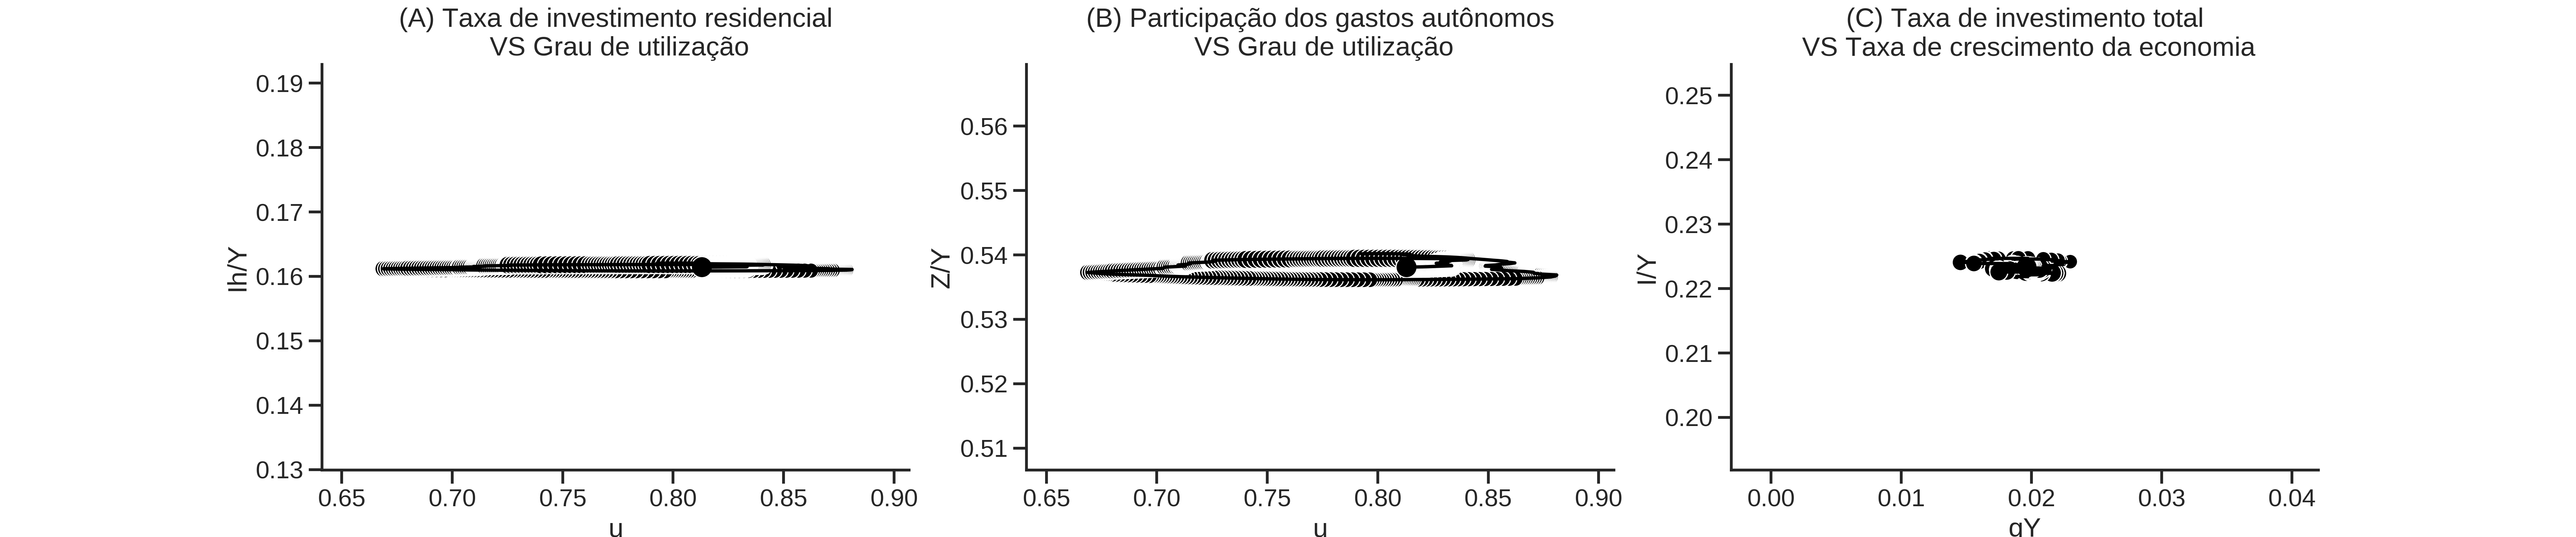
\includegraphics[width=\textwidth]{../../Modelo/Versoes/Clock_Real.png}
	\caption*{\textbf{Fonte:} Elaboração própria}
\end{figure}


Uma breve inspeção do gráfico \ref{clock_Real} explicita a relação cíclica e horária entre participação dos gastos autônomos e nível de atividade tal como discutido no capítulo anterior e o mesmo pode ser dito a respeito da taxa de investimento residencial e grau de utilização. Já o fato estilizado (1) não apresenta um padrão tão demarcado\footnote{A dificuldade de explicitar um padrão bem demarcado também decorre da volatilidade elevada de um dos eixos (taxa de crescimento) enquanto o outro é menos volátil (taxa de investimento).} uma vez que apresenta uma relação positiva entre taxa de investimento e de crescimento em alguns subperíodos e negativa em outros.

\begin{figure}[H]
	\centering
	\caption{Inserindo Taxa Própria, taxa de juros hipotecária e inflação de móveis observada}
	\label{choque_Real}
	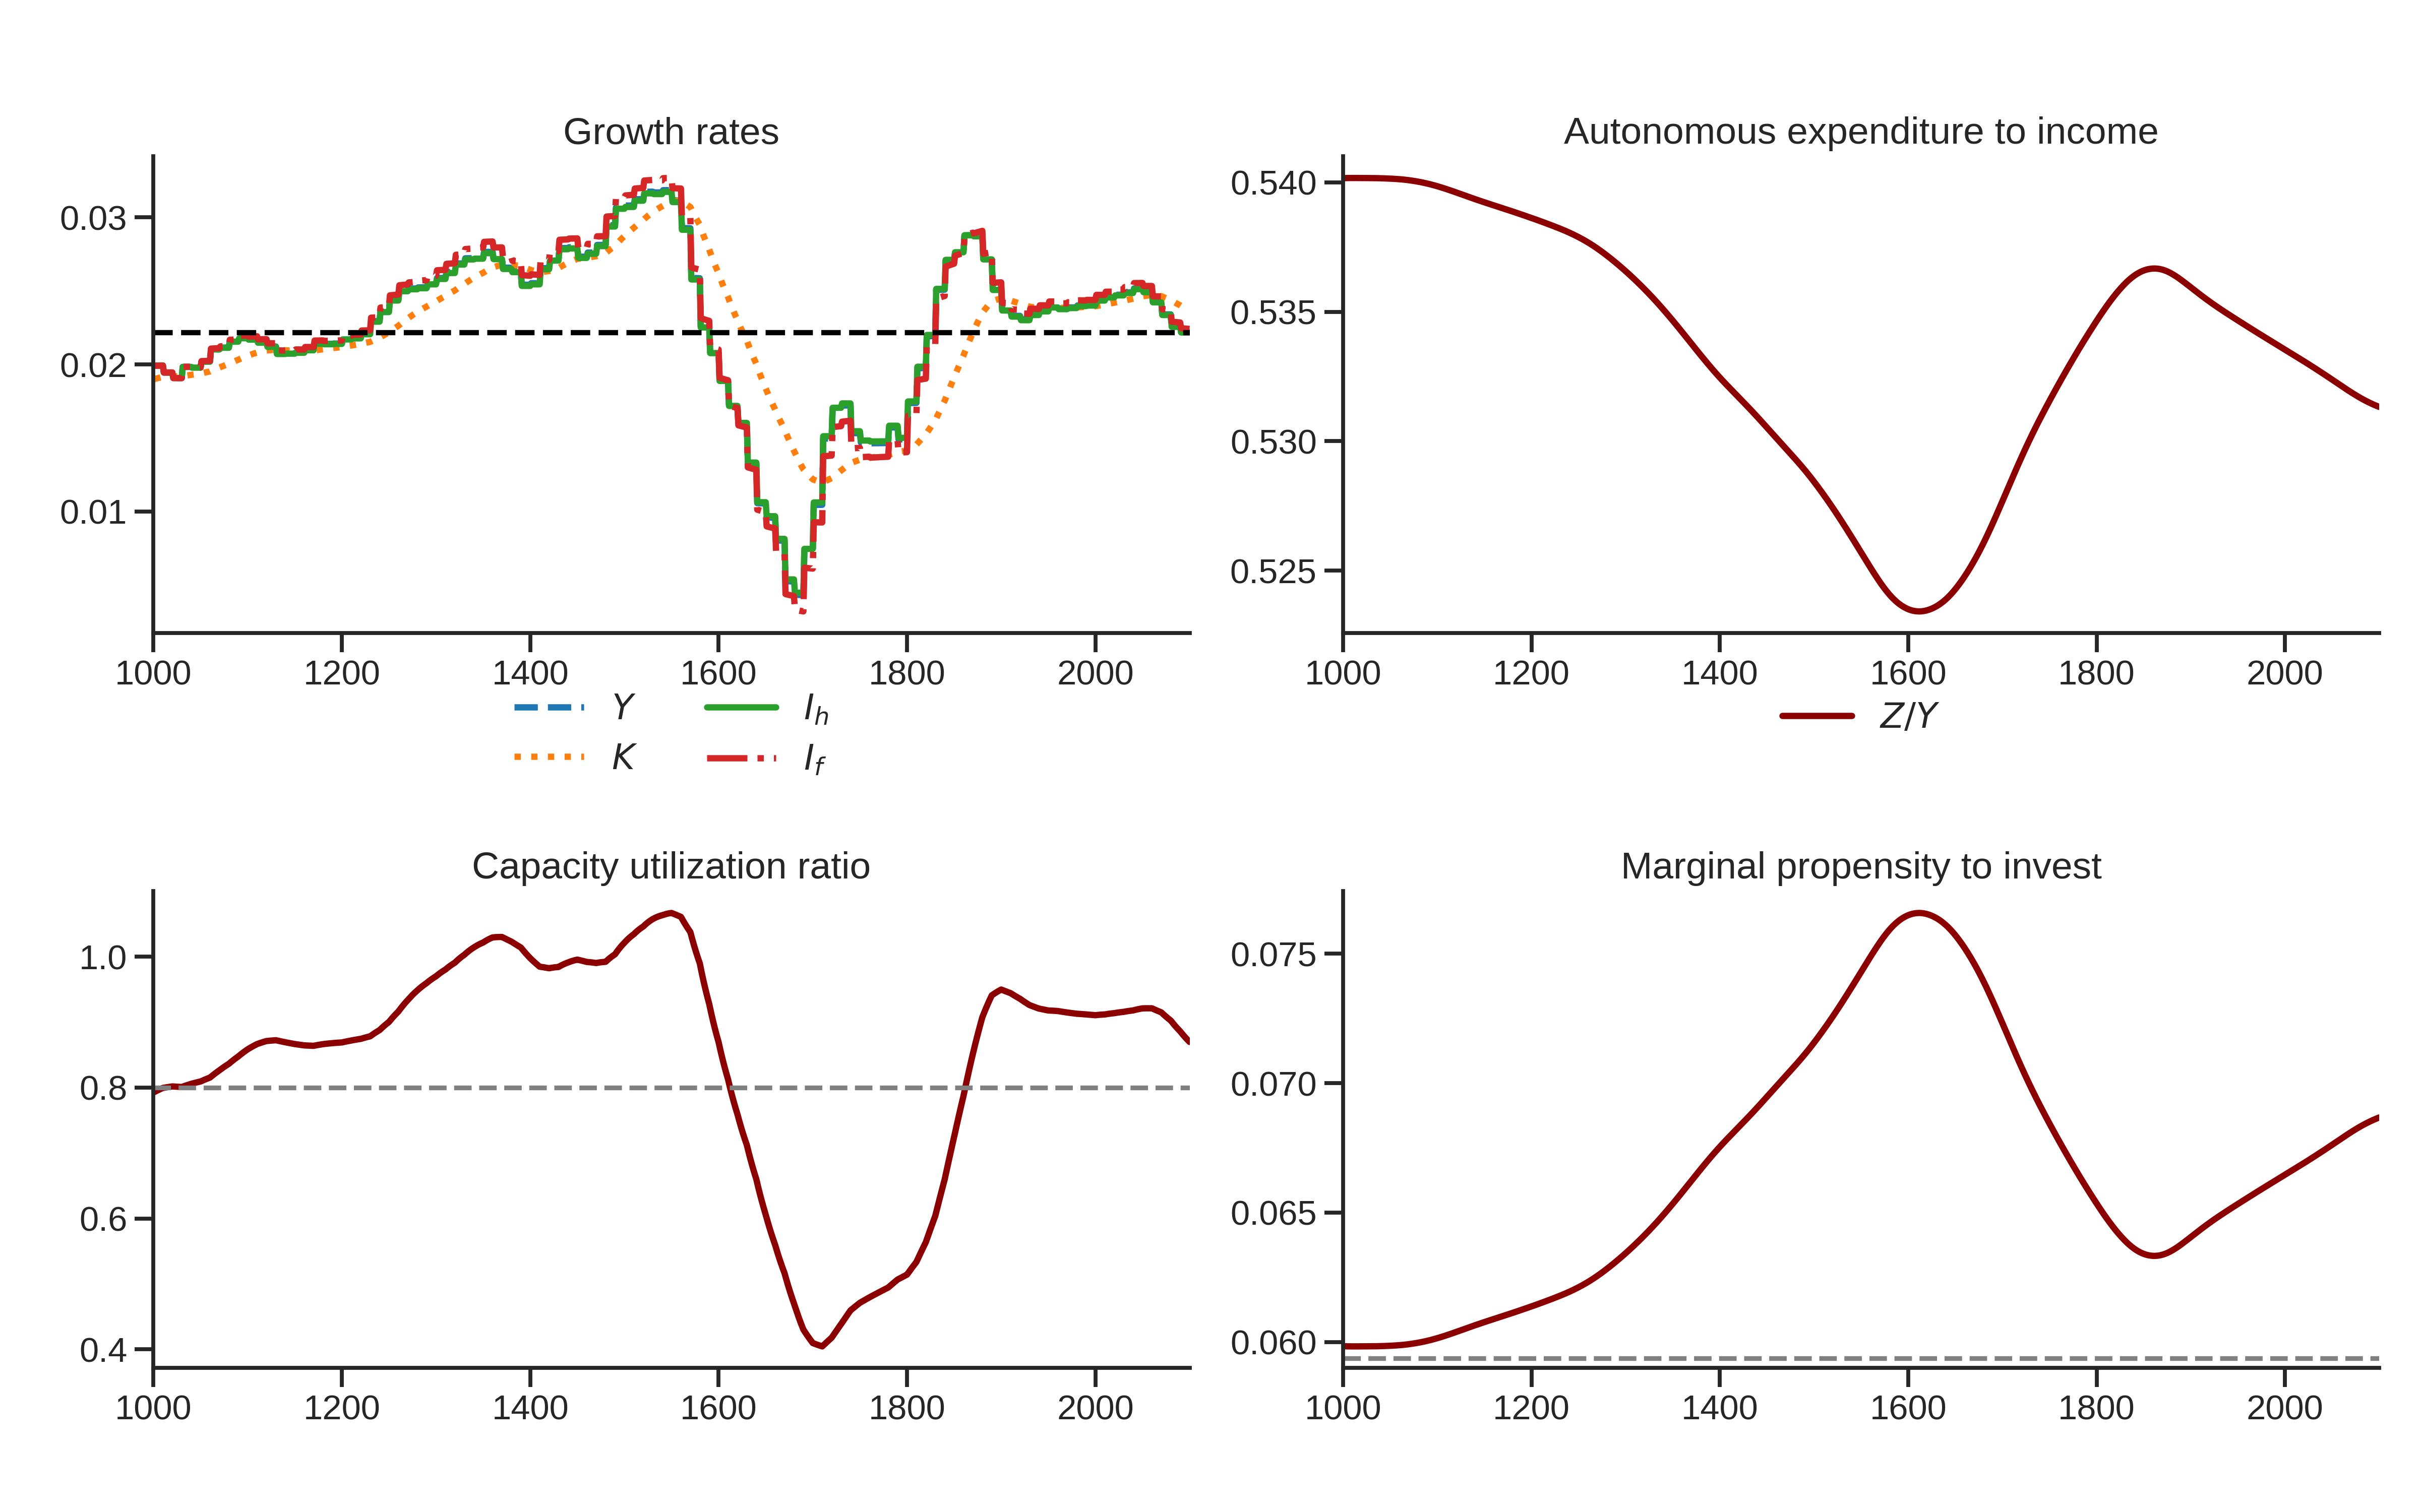
\includegraphics[width=\textwidth]{../../Modelo/Versoes/Shock_Real.png}
	\caption*{\textbf{Fonte:} Elaboração própria}
\end{figure}


O fato estilizado (2) referente ao grau de utilização é contemplado --- feitas as devidas mediações --- uma vez que o período analisado não corresponde a posição plenamente ajustada e, portanto, desvios no grau de utilização em relação ao normal são ajustados por meio de mudanças na propensão marginal a investir (fato estilizado 6). Por fim, destaca-se o acompanhamento da taxa de crescimento da economia aos gastos autônomos, notadamente investimento residencial. No entanto, não é capaz de replicar o fato estilizado (5) de maior volatilidade do investimento residencial.

\begin{figure}[H]
	\centering
	\caption{Inserindo Taxa Própria, taxa de juros hipotecária e inflação de móveis observada}
	\label{choque_RealNorms}
	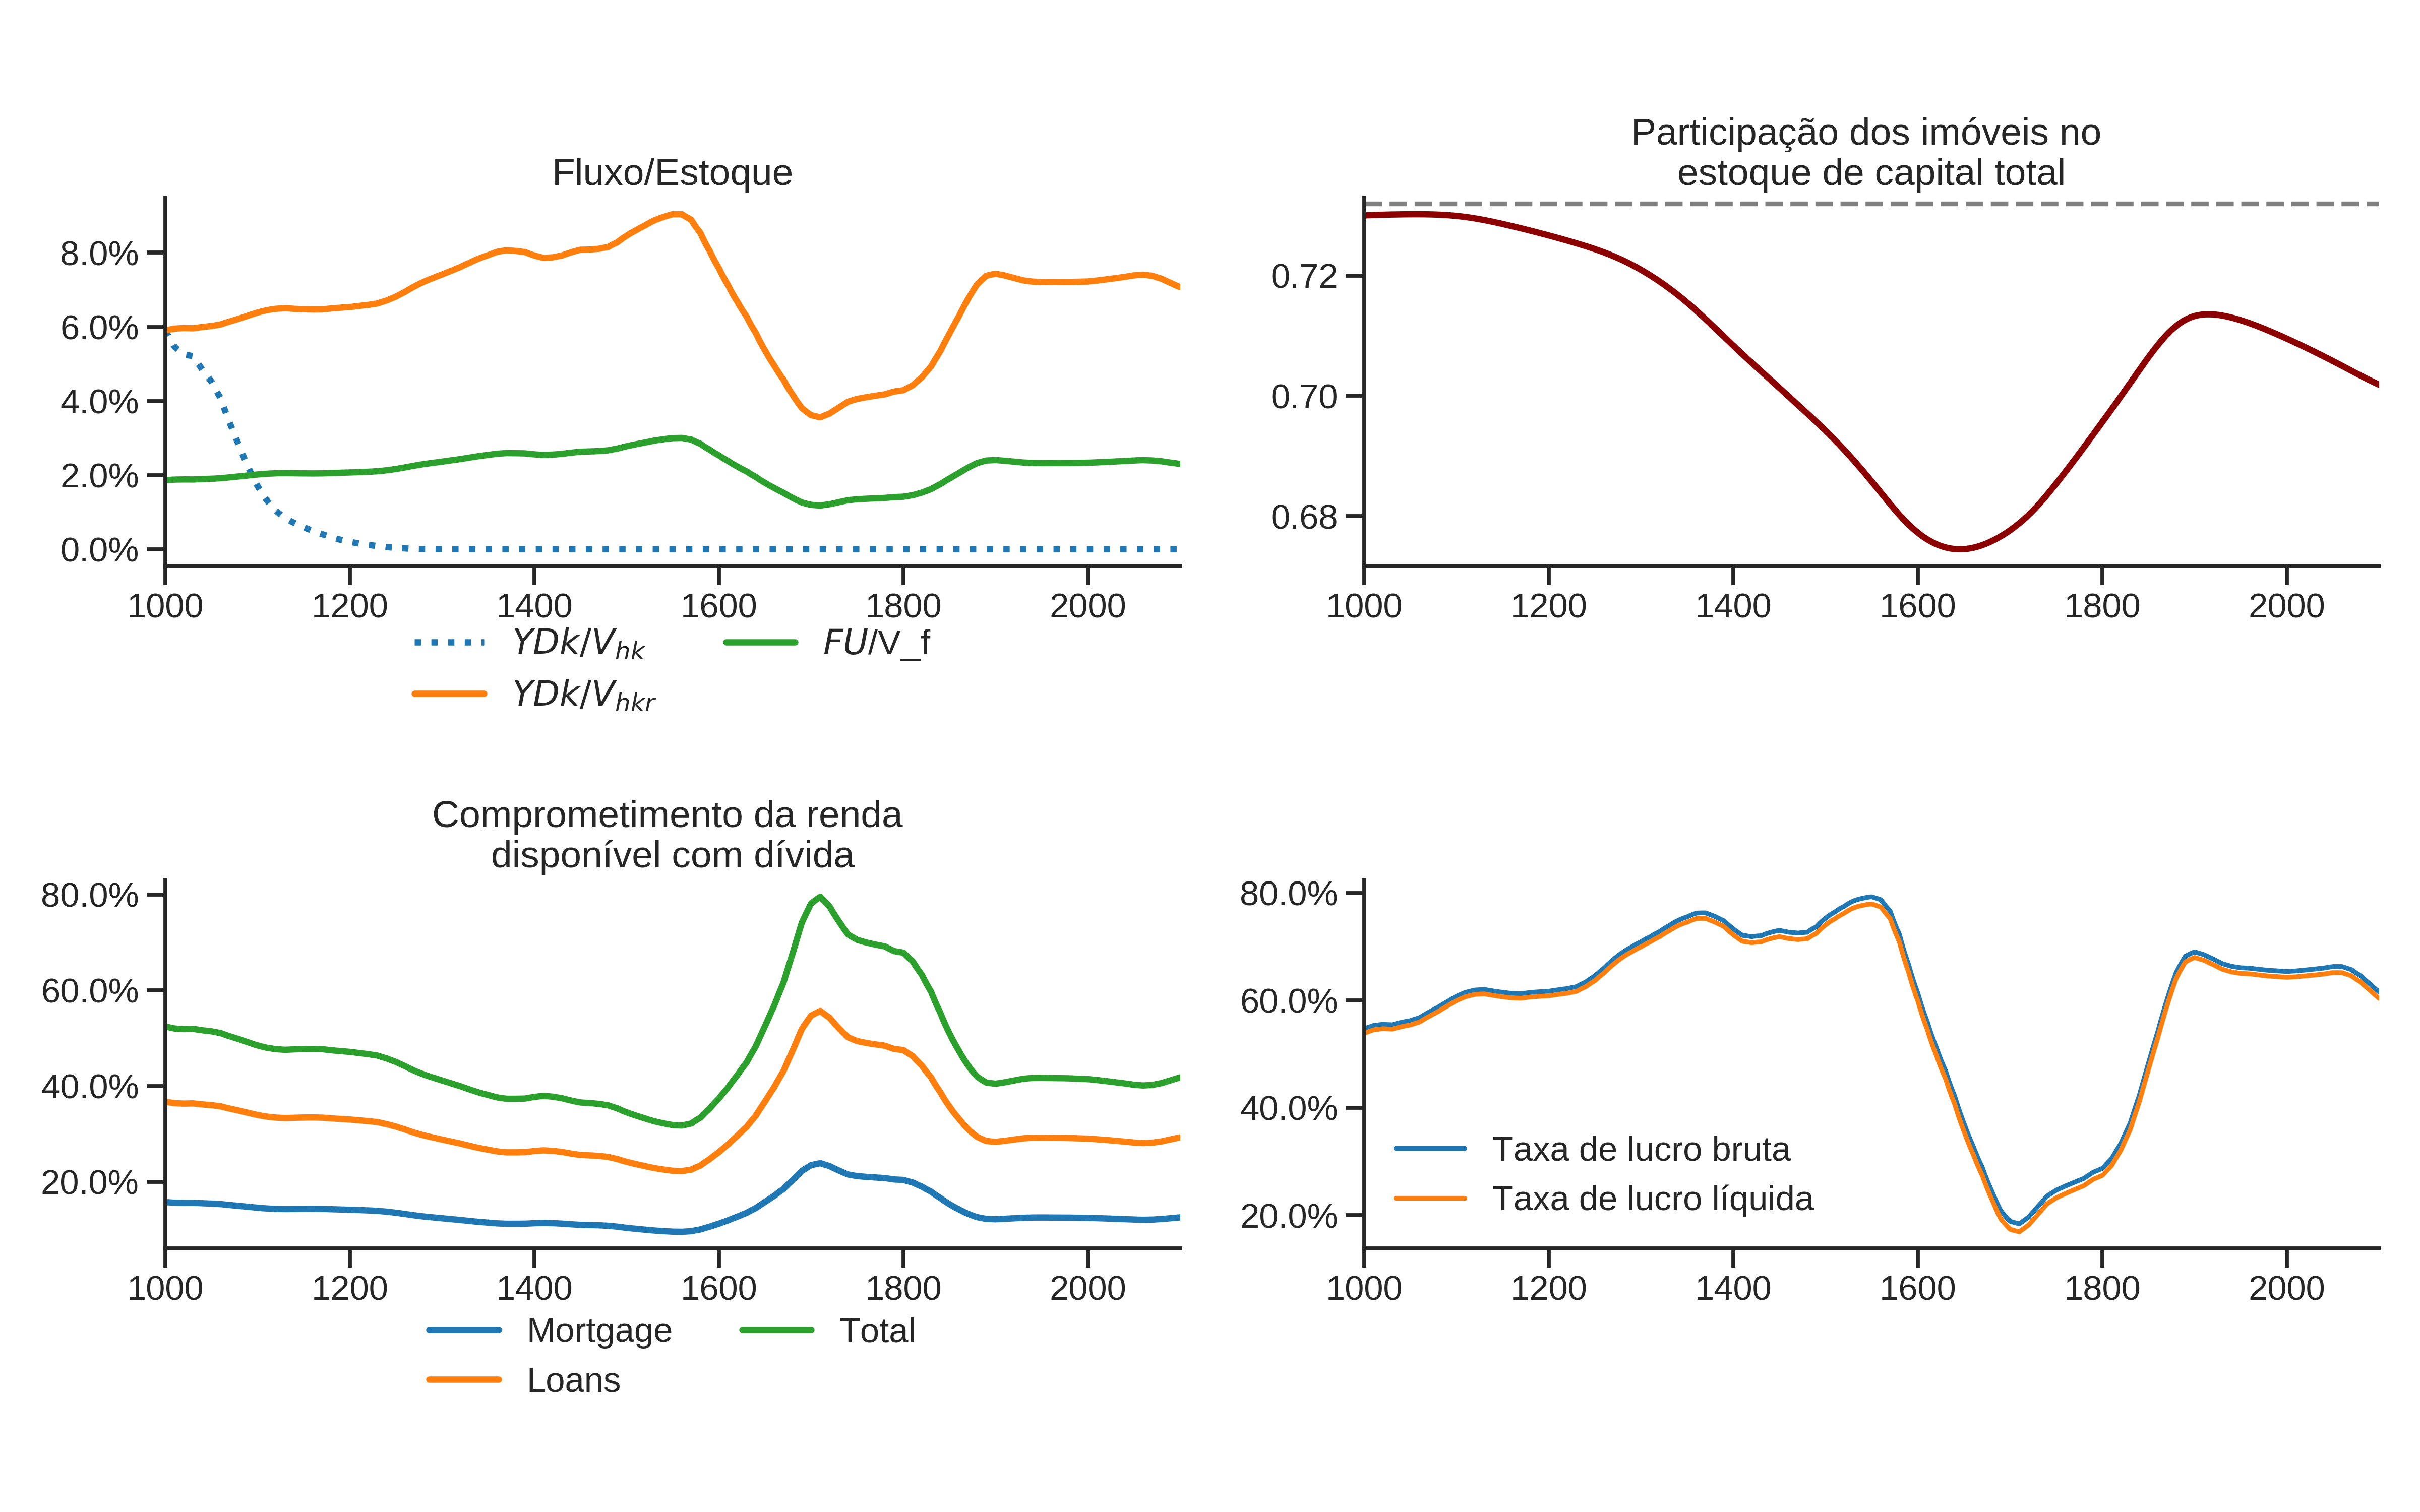
\includegraphics[width=\textwidth]{../../Modelo/Versoes/Shock_RealNorms.png}
	\caption*{\textbf{Fonte:} Elaboração própria}
\end{figure}

Por fim, destaca-se a reprodução do fato estilizado (3) em que tanto o comprometimento da renda das famílias com o pagamento de juros aumenta quanto a razão entre renda disponível em relação a riqueza diminui. Tal dinâmica de endividamento não teve um paralelo nas firmas uma vez que a taxa de lucro bruta e líquida se aproximaram no período equivalente a crise. Além disso, esta simulação reproduz a redução nas taxas de lucro ao longo da crise que está associada a redução do nível de atividade --- dada a participação dos lucros na renda constante.

Vale lembrar que este é um primeiro esforço de confrontar um modelo teórico simulado com investimento residencial frente aos dados observados.
Além disso, tal procedimento não conta com a calibragem dos parâmetros e esta é uma frete de melhoria que versões futuras desta pesquisa pode seguir.
No entanto, os problemas decorrentes desta primeira tentativa de mediação entre teoria e empiria não se restrigem à calibragem. 
Apesar de lançar luz sobre alguns pontos destacados pela teoria, deixa outros em aberto e que devem ser aprimorados preservando as hipóteses do modelo:
\begin{description}
	\item[Temporalidade] Normalmente não é feita uma distinção/discussão nos modelos do tipo SFC de simulação sobre o significado econômico das defasagens adotadas. Sendo assim, para que um modelo teórico tenha maior aderência a empiria é preciso repensar o significado da temporalidade de algumas variáveis;
	\item[Grau de utilização normal] Ao longo desta pesquisa, adotou-se um grau de utilização normal arbitrário (e constante) que, por sua vez, não equivale --- necessariamente --- à média ou à tendência do grau de utilização efetivo. Desse modo, é preciso avançar em direção às formas de incluir tal conceito nos modelos sem incorrer em imprecisões teóricas nem se restringir a arbitrariedade;
	\item[Participação dos gastos autônomos] Tal como o grau de utilização normal, a escolha da participação dos gastos autônomos ($R$) também é arbitrária. Se faz necessário investigar formas de endogeneizar tal participação sem incorrer em soluções assintóticas em que a parcela de um dos gastos converge a zero;
	\item[Saldo líquido dos setores] Por se tratar de uma economia fechada sem governo, se as famílias forem deficitárias neste modelo as firmas serão necessariamente superavitárias (e o inverso também é válido).
	Sendo assim, para que esta dualidade não seja a única combinação possível se faz necessário incluir outros setores institucionais. No entanto, versões futuras desta pesquisa irão avançar neste nível de complexidade se acrescentar elementos relevantes tanto para a dinâmica do investimento residencial quanto para as implicações macroeconômicas deste gasto. Caso contrário, tais modificações adicionarão complexidade sem incluir --- necessariamente --- maior esclarecimento;
	\item[Composição do patrimônio líquido dos bancos] Ao longo deste capítulo adotou-se a hipótese que os bancos não auferem lucros e, por consequência, não acumulam ativos.
	Sendo assim, tal modelo não consegue reproduzir --- por construção --- razões entre ativos/passivos sobre o patrimônio líquido uma vez que a riqueza (total e financeira) deste setor institucional é nula.
	Desse modo, para que seja capaz de replicar mudanças na composição do patrimônio líquido dos bancos é preciso que este setor passe a obter lucros que, por sua vez, rompe com as hipóteses aqui adotadas.
\end{description}

Apesar destas questões que precisam ser melhor desenvolvidas, pontua-se que 
esta pesquisa contribuiu para a literatura de crescimento liderado pela demanda do modelo do supermultiplicador sraffiano, levando em consideração o esforço recente de incorporá-lo em um arcabouço contábil do tipo SFC.  A característica específica do modelo aqui apresentado é a inclusão do investimento residencial. A introdução desse gasto teve como objetivo dar conta dos resultados de alguns trabalhos empíricos recentes que mostram a importância do investimento residencial para dinâmica macroeconômica e, como visto anteriormente, nenhum trabalho havia simulado esse gasto específico via taxa própria de juros dos imóveis. 

O modelo reproduz as principais características do supermultiplicador sraffiano: (i) o grau de utilização converge ao grau normal, por meio de variações da propensão marginal a investir das firmas e; (ii) a taxa de crescimento da economia segue a taxa de crescimento dos gastos autônomos --- nesse caso, o investimento residencial. A primeira diferença do  presente modelo é que o estoque de capital fixo da economia passa a ter dois componentes, o capital produtivo das firmas e os imóveis das famílias. 

Como visto nas simulações, o principal resultado particular deste modelo é que uma maior taxa de crescimento do investimento residencial tem como consequência uma redução da participação do estoque de imóveis no capital total. Tal resultado, aparentemente contra intuitivo, se deve ao ajuste do estoque de capital das firmas. Para que o grau efetivo de utilização da capacidade convirja ao grau normal, o investimento das firmas precisa temporariamente crescer mais rápido que investimento residencial, alterando, portanto, a relação entre os dois estoques. 

Os outros dois experimentos trazem resultados em linha com o supermultiplicador sraffiano. A diminuição da participação dos salários na renda não afeta a taxa de crescimento de longo prazo e, portanto, não afeta a propensão marginal a investir de forma permanente. Porém, por alterar o tamanho do supermultiplicador, diminui a participação do capital produtivo no capital total. O aumento da taxa de juros, por sua vez, tem um efeito tanto sobre a taxa de crescimento de longo prazo quanto sobre o endividamento das famílias em relação à renda disponível. 

É importante destacar que este trabalho é apenas o primeiro passo numa agenda de pesquisa mais ampla sobre o papel do investimento residencial no ciclo e no crescimento econômico. Pesquisas futuras podem (e devem) tornar o modelo aqui apresentado mais complexo. Possíveis extensões incluem explorar outros determinantes do investimento residencial bem como seus impactos sobre outros gastos autônomos, sobre o colateral das famílias e patrimônio líquido dos bancos.
Com isso, concluí-se os objetivos pretendidos com o modelo apresentado. Cabe ao capítulo seguinte reunir as conclusões desta pesquisa e alguns direcionamentos futuros.
